\section{Multi-class SVM}

\mode<presentation>{
\begin{frame} 
    \begin{center} \huge
        \secname
    \end{center}
    \begin{center}
    A very brief overview   
    \end{center}
\end{frame}
}

\begin{frame}\frametitle{The binary classification setting}

\mode<article>{
\underline{The binary classification setting}:\\
}

Classification problems have labels with only finitely many possible values.

Example: Binary classification, $y_{T} \in \{-1,1\}$:

\begin{figure}[ht]
     \centering
     \savebox{\imagebox}{
	 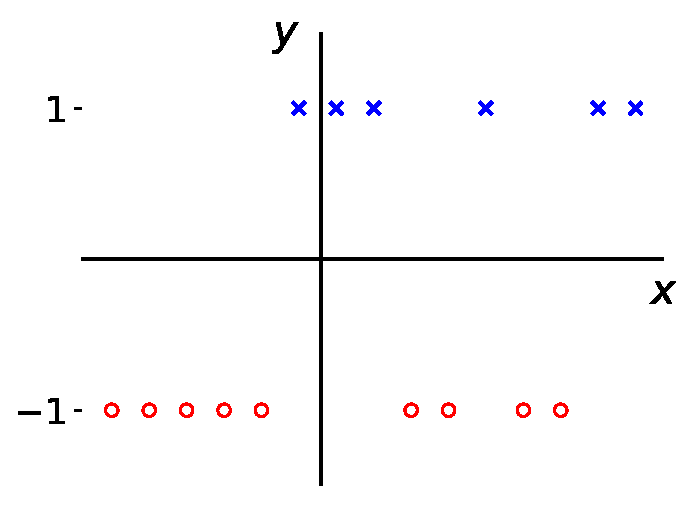
\includegraphics[width=0.35\textwidth]{img/classification_1d_sign}}%
     \begin{subfigure}[t]{0.35\textwidth}
         \centering
         \usebox{\imagebox}% Place largest image
         \caption{1D input}
         \label{fig:classification1d}
     \end{subfigure}
     \hspace{10mm}
     \begin{subfigure}[t]{0.35\textwidth}
         \centering
         \raisebox{\dimexpr.5\ht\imagebox-.5\height}{% Raise smaller image into place
         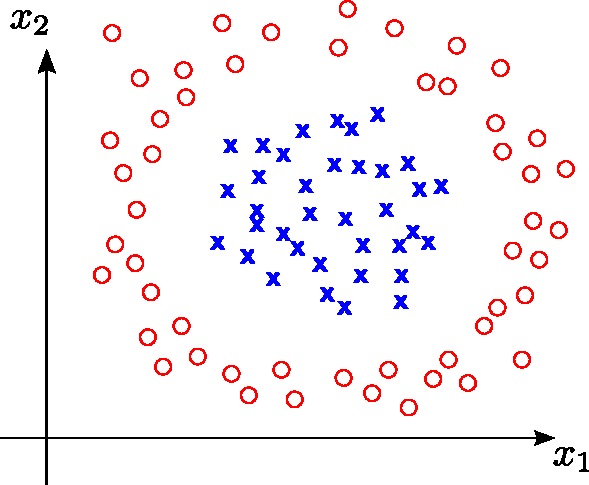
\includegraphics[width=0.99\textwidth]{img/circular}
         }
         \caption{2D input}
         \label{fig:classification2d}
     \end{subfigure}
     \caption{binary classification}
	 \label{fig:classification}
\end{figure}

\end{frame}

\begin{frame}\frametitle{The multi-class classification setting}

A set of $K>2$ classes: $\{c_{1},c_{2},\ldots,c_{K}\}$

\begin{figure}[h]
     \centering
	 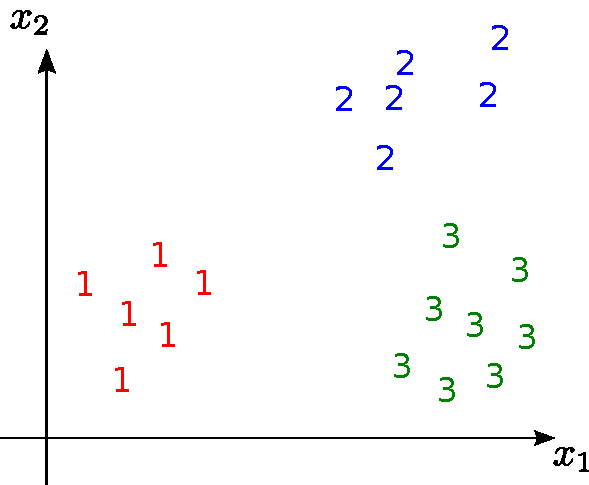
\includegraphics[width=0.35\textwidth]{img/3classes}
     \caption{multi-class classification}
	 \label{fig:multiclassification}
\end{figure}

Remains an open issue for SVMs.

\end{frame}

\subsection{One-vs-rest (one-vs-all)}

\begin{frame}\frametitle{\subsecname}

\only<1-3>{
\begin{itemize}
\item[] for each class $c_{k}$ in $\{c_{1},c_{2},\ldots,c_{K}\}$\\
do
\begin{itemize}
\item[] train a binary classifier with $c_{k}$ as its \textbf{positive} class
\item[] \textbf{all} remaining $K-1$ classes are treated collectively as the \textbf{negative} class.\\
\end{itemize}
end
\end{itemize}

\slidesonly{
\only<1>{
%\textbf{see blackboard}
\begin{center}
	 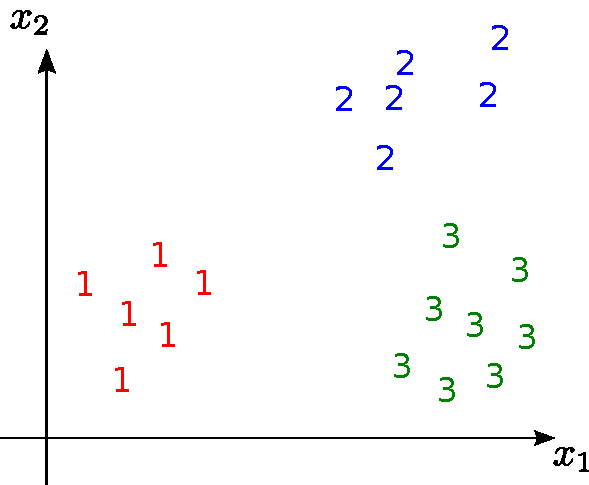
\includegraphics[width=4cm]{img/3classes}
\end{center}
}
}

}
\only<2->{

\svspace{-5mm}
%\slidesonly{
	%\begin{textblock}{}(10,5)
%}
\begin{center}
	 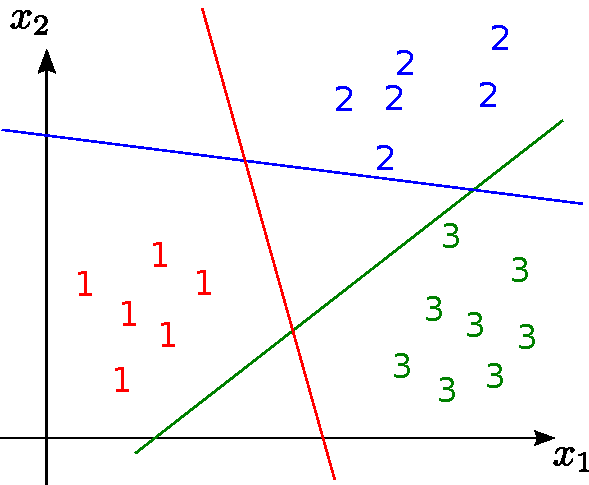
\includegraphics[width=4cm]{img/3classes_onevsall}
     \captionof{figure}{$K$ one-vs-all classifiers}
	 \label{fig:multiclassification}
\end{center}
%\slidesonly{
	%\end{textblock}
%}

\svspace{-5mm}
\only<3>{
\question{Any potential problems with training $K$ one-vs-all classifiers?}
}
}

\only<4>{
\svspace{-3mm}

\begin{itemize}
\item ambiguous regions
\item needs heuristic to disambiguate (e.g. $\argmax_{k} y_{k}(\vec x)$)\\
    but any heuristic needs to deal with the different scales of each $y_{k}(\vec x)$
\item each classifier faces an imbalanced training set. \notesonly{In the case of SVMs, this leads to asymmetric margins.} 
But ``class weighted'' SVMs exist.
\end{itemize}

Actually: one-vs-rest classification for SVMs is good enough for many problems.
}

    
\end{frame}

\mode<article>{
%\begin{frame}

\begin{figure}[h]
     \centering
	 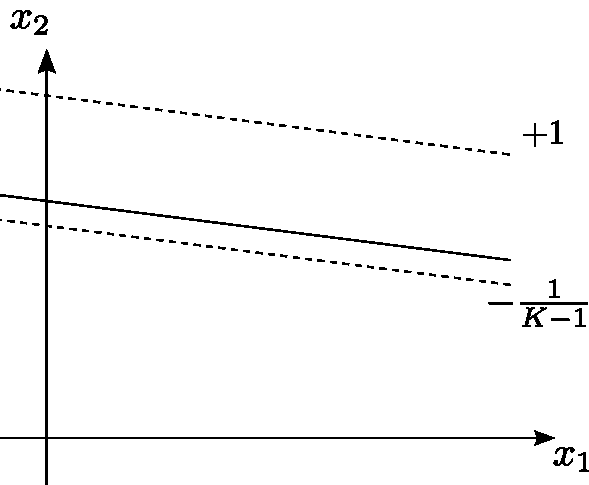
\includegraphics[width=4cm]{img/asymmetric}
     \caption{Asymmetric margins due to class imbalance}
	 \label{fig:imbalance}
\end{figure}

%Actually: one-vs-rest classification for SVMs is good enough for many problems.

    
%\end{frame}
}

\subsection{One-vs-one (all pairs)}

\begin{frame}\frametitle{\subsecname}

\# binary classifiers = $\frac{K(K-1)}{2}$ 

\begin{itemize}
\item[:-(] long test times.\\
    Testing speed can be improved by organizing the pair classifiers into a DAG\footnote{Directed Acyclic Graph, a tree would qualify.} to reduce to a subset of $K-1$ only.
\item[:-)] Training is fast as each only requires a very small subset of the data. 
\item[:-(] We still have ambiguous regions:    
\end{itemize}

\begin{center}
	 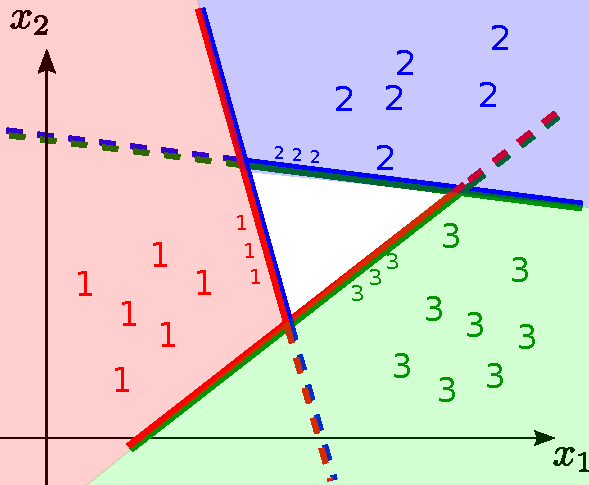
\includegraphics[width=4.8cm]{img/3classes_onevsone_majority}
	 \mode<article>{
     \captionof{figure}{One-vs-one classification}
     }
	 \label{fig:onevsone}
\end{center}
    
\end{frame}

\subsection{Binary classification with error-correcting outputs}

\begin{frame}{\subsecname}

A rough outline of this ensemble method:

\begin{enumerate}
\item Express each class using an $L$-bit binary vector (e.g. $\{+1,-1\}$). Choose $L>K$.
\item Concatenate all vectors into a $K \times L$ matrix. 
\item Train a binary classifier to target the value of the $i$-th column in this matrix.
    \begin{itemize}
    \item If class $k$ is associated with a ``$+1$'' at the $i$-th column. All data from this class will be used as \textbf{positive} examples when training the $i$-th classifier.
    \item If class $k$ is associated with a ``$-1$'' at the $i$-th column. All data from this class will be used as \textbf{negative} examples when training the $i$-th classifier.
    \end{itemize}
\end{enumerate}
    
\end{frame}

\begin{frame}\frametitle{Example for error correcting codes}

% Please add the following required packages to your document preamble:
% \usepackage{graphicx}
\begin{table}[]
%\resizebox{\textwidth}{!}
{%
\begin{tabular}{|c|c|c|c|c|c|c|}
\hline
Class & $l_1$ & $l_2$ & $l_3$ & $l_4$ & $l_5$ & $l_6$ \\ \hline\hline
$c_{1}$ & 1 & -1 & 1 & -1 & -1 & 1 \\ \hline
$c_{2}$ & 1 & 1 & -1 & -1 & 1 & -1 \\ \hline
$c_{3}$ & -1 & 1 & -1 & 1 & -1 & 1 \\ \hline
$c_{4}$ & -1 & -1 & 1 & -1 & 1 & 1 \\ \hline
\end{tabular}%
}
\caption{Example for error correcting codes using 6-bits for 4 classes}
\end{table}

Classifier $y_{2}(\vec x)$ will use all points from $c_{2}$, $c_{3}$ as positive examples and $c_{1}$, $c_{4}$ as negative examples.

By looking at the predictions of all classifiers. One would match the $6$-bit prediction pattern with those of the 4 classes to determine which class was detected.

\end{frame}
